%%%%%%%%%%%%%%%%%%%%%%%%%%%%%%%%%%%%%%%%%
% Beamer Presentation
% LaTeX Template
% Version 1.0 (10/11/12)
%
% This template has been downloaded from:
% http://www.LaTeXTemplates.com
%
% License:
% CC BY-NC-SA 3.0 (http://creativecommons.org/licenses/by-nc-sa/3.0/)
%
%%%%%%%%%%%%%%%%%%%%%%%%%%%%%%%%%%%%%%%%%

%----------------------------------------------------------------------------------------
%	PACKAGES AND THEMES
%----------------------------------------------------------------------------------------

\documentclass{beamer}

\mode<presentation> {

% The Beamer class comes with a number of default slide themes
% which change the colors and layouts of slides. Below this is a list
% of all the themes, uncomment each in turn to see what they look like.

%\usetheme{default}
%\usetheme{AnnArbor}
%\usetheme{Antibes}
%\usetheme{Bergen}
%\usetheme{Berkeley}
%\usetheme{Berlin}
%\usetheme{Boadilla}
%\usetheme{CambridgeUS}
%\usetheme{Copenhagen}
%\usetheme{Darmstadt}
%\usetheme{Dresden}
%\usetheme{Frankfurt}
%\usetheme{Goettingen}
%\usetheme{Hannover}
%\usetheme{Ilmenau}
%\usetheme{JuanLesPins}
%\usetheme{Luebeck}
\usetheme{Madrid}
%\usetheme{Malmoe}
%\usetheme{Marburg}
%\usetheme{Montpellier}
%\usetheme{PaloAlto}
%\usetheme{Pittsburgh}
%\usetheme{Rochester}
%\usetheme{Singapore}
%\usetheme{Szeged}
%\usetheme{Warsaw}

% As well as themes, the Beamer class has a number of color themes
% for any slide theme. Uncomment each of these in turn to see how it
% changes the colors of your current slide theme.

%\usecolortheme{albatross}
%\usecolortheme{beaver}
%\usecolortheme{beetle}
%\usecolortheme{crane}
%\usecolortheme{dolphin}
%\usecolortheme{dove}
%\usecolortheme{fly}
%\usecolortheme{lily}
%\usecolortheme{orchid}
%\usecolortheme{rose}
%\usecolortheme{seagull}
%\usecolortheme{seahorse}
%\usecolortheme{whale}
%\usecolortheme{wolverine}

%\setbeamertemplate{footline} % To remove the footer line in all slides uncomment this line
%\setbeamertemplate{footline}[page number] % To replace the footer line in all slides with a simple slide count uncomment this line

%\setbeamertemplate{navigation symbols}{} % To remove the navigation symbols from the bottom of all slides uncomment this line
}

\usepackage{graphicx} % Allows including images
\usepackage{booktabs} % Allows the use of \toprule, \midrule and \bottomrule in tables
\usepackage{tikz}
\usepackage[utf8]{inputenc}

%----------------------------------------------------------------------------------------
%	TITLE PAGE
%----------------------------------------------------------------------------------------

\title[Betweenness Centrality]{Betweenness Centrality} % The short title appears at the bottom of every slide, the full title is only on the title page

\author{Max Kießling, Wolfgang Otto, Sören Reichardt} % Your name
\institute[UL] % Your institution as it will appear on the bottom of every slide, may be shorthand to save space
{
Unitversität Leipzig \\ % Your institution for the title page
\medskip
\textit{} % Your email address
}
\date{\today} % Date, can be changed to a custom date

\begin{document}

\begin{frame}
\titlepage % Print the title page as the first slide
\end{frame}

%----------------------------------------------------------------------------------------
%	PRESENTATION SLIDES
%----------------------------------------------------------------------------------------

\begin{frame}
\frametitle{Thema}
\centering
Umsetzung der Berechnung des Betweenness Centrality Maßes \\
im Big Data Umfeld
\end{frame}

\begin{frame}
\frametitle{Was ist Betweenness Centrality?}
\begin{itemize}
\item Mass der Zentralität eines Knotens:
	\begin{itemize}
	\item entspricht der Anzahl der kürzesten Wege zwischen allen Paaren von Knoten, die durch den betrachteten Knoten führen
	\end{itemize}
\item Knoten mit hohen Zentralitätswerten haben großen Einfluss auf das Netzwerk
\item wird häufig zur Analyse sozialer Netzwerke verwendet
	

\end{itemize}
\end{frame}

%------------------------------------------------

\begin{frame}
\frametitle{Was ist Betweenness Centrality?}
\begin{figure}[h]
	\centering
	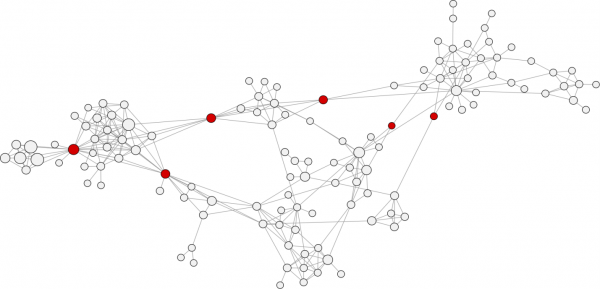
\includegraphics[width=10cm]{images/bc-example}
\end{figure}
\end{frame}
%------------------------------------------------
\begin{frame}
\frametitle{Berechnung - Idee}
\begin {itemize}
	\item Zwei Schritte:
	 \begin{itemize}
	 	\item Berechnung aller kürzesten Pfade
	 	\item Für jeden Knoten zählen, auf wieviel kürzesten Pfaden er liegt
	 \end {itemize}
	\item Iterativer Ansatz
	\begin{itemize}
		\item Berechnung der kürzesten Pfade von jedem Ausgangsknoten
	 	\item Berechnung der Betweenness Centrality relativ zu jedem dieser Ausgangsknoten
	 	\item Aufsummieren der Werte
	\end {itemize}
	\item Innovation des von Ulrik Brandes vorgestellten Algorithmus:
	\begin{itemize}
		\item Zur Berechnung eines Wertes für einen Knoten ist nicht das Wissen über komplette Pfade notwendig
		\item Denn: Liegt Knoten A auf dem kürzesten Pfad zu Knoten B, so liegt Knoten A auch auf allen kürzesten Pfaden auf denen B liegt
		\item Idee: Aufsummieren der Werte der Nachfolger
	 \end{itemize}
\end {itemize}
\end{frame}
%------------------------------------------------

\begin{frame}
\frametitle{Algorithmus: Betweenness Centrality}
\begin{itemize}
\item Algorithmus besteht grob aus zwei Schritten:
	\begin{enumerate}
	\item modifiziertes Single Source Shortest Paths
		\begin{itemize}
		\item Knoten speichern zusätzlich alle direkten Vorgänger
		\end{itemize}
	\item ``einsammeln der Daten''
		\begin{itemize}
		\item Ausgehend von den entferntesten Knoten:
		\item verschicken von Nachrichten an alle Vorgänger 
		\item Bsp.: bei 2 Vorgängern verschickt ein Knoten \(1  / Anzahl Vorgaenger\) , also \(1/2\) an beide Vorgängerknoten
		\end{itemize}
	\end{enumerate}
\item dieser Prozess wird für alle Knotenpaare wiederholt, sowie die entstehenden Zentralitätswerte für jeden Knoten aufsummiert
\end{itemize}
\end{frame}
%------------------------------------------------
\begin{frame}
\frametitle{Unser Vorgehen bei der Umsetzung des Algorithums in einer Big Data Architektur}
\begin{enumerate}
\item Ausprobieren von Flink Gelly und Spark GraphX durch implementierung von SSSP in beiden Frameworks
\item Implementierung der Berechungung der Betweenness Centrality in Spark GraphX
\item Implementierung einer Berechnungsalternative, die die Nachrichtenzahl reduziert
\item Testorientiertes Vorgehen
\end{enumerate}
\end{frame}

%------------------------------------------------
\begin{frame}
\frametitle{Implementierung}
\begin{itemize}
\item Implementierung mittels \textit{Spark Graphx} in Scala
\item Apache Spark ist ein Open Source Framework zur verteilten Analyse großer Datenmengen
\item die Hauptmerkmal von Spark sind \textit{resilient distributed datasets (RDD)}, verteilte Mengen von Elementen und vordefinierten parallelen Operationen
\end{itemize}
\end{frame}

%------------------------------------------------

\begin{frame}
\frametitle{GraphX}
\begin{itemize}
\item \textit{GraphX} ist eine API von Apache Spark für (parallele) Berechnungen auf Graphen
\item Unterstützt ein Google Pregel ähnliches Programmiermodell für iterative Berechnungen auf Graphen
\item Pregel ist eine \textit{bulk-synchronous parallel messaging} Abstraktion
	\begin{itemize}
	\item Knotenbasierte Sichtweise (``think like a vertex'')
	\item Ausführung erfolgt in Supersteps
	\item ein Programm besteht aus 3 Funktionen:
		\begin{enumerate}
		\item Vertex Program
		\item Send Messages
		\item Merge Messages
		\end{enumerate}
	\end{itemize}

	
\end{itemize}
\end{frame}

%------------------------------------------------

\begin{frame}
\frametitle{Ausblick}
\begin{itemize}
\item Fehleranalyse sowie Test auf großem Cluster
\item Optimierung des Speicherbedarfs / Laufzeit
\end{itemize}
\end{frame}

%------------------------------------------------

\begin{frame}
\frametitle{Lessons Learned}
\begin{itemize}
\item Einstieg in das Programmieren mit Scala
\item Einstieg in zwei Graph Processing Frameworks im Big Data Umfeld
\item Tieferes Verständnis für die Adaption von Algorithmen in praktische Umgebungen
\item Bewältigung von Problemen die das Spark Datenflussmodell mit sich bringt
\end{itemize}
\end{frame}

\begin{frame}
\frametitle{References}
\footnotesize{
\begin{thebibliography}{99} % Beamer does not support BibTeX so references must be inserted manually as below

\bibitem[Brandes, 2001]{p2} Ulrik Brandes(2001)
\newblock A Faster Algorithm for Betweenness Centrality
\newblock \emph{URL} http://algo.uni-konstanz.de/publications/b-fabc-01.pdf
\end{thebibliography}
}
\end{frame}

%----------------------------------------------------------------------------------------

\end{document} 